\documentclass[a4paper,11pt,final]{article}
\usepackage[scaled=0.9]{luximono}
\usepackage[spanish]{babel}
\usepackage[utf8]{inputenc}
\usepackage[T1]{fontenc}
\usepackage{booktabs}
\usepackage{epstopdf}
\usepackage{graphicx}
\usepackage{hyperref}
\usepackage{multicol}
\usepackage{tabularx}
\usepackage{textcomp}
\usepackage{amsmath}
\usepackage{amssymb}
\usepackage{amstext}
\usepackage{charter}
\usepackage{amsbsy}
\usepackage{amsthm}
\usepackage{lipsum}
\usepackage{natbib}
\usepackage{array}
\usepackage{color}
\usepackage{esint}
\usepackage{float}

% Hyperref setup
\hypersetup{pdftitle={Procesamiento de datos digitales. Laboratorio 1},
            pdfauthor={César Jiménez Tintaya},
            pdfpagelayout=OneColumn,
            pdfnewwindow=true,
            pdfdisplaydoctitle=true,
            pdfstartview=XYZ,
            plainpages=false,
            unicode=true,
            bookmarksnumbered=true,
            bookmarksopen=true,
            bookmarksopenlevel=3,
            breaklinks=true,
            colorlinks=true,
            linkcolor=blue,
            pdfborder={0 0 0}}

%% LaTeX commands.
\makeatletter
%% -----------------------------------------------------------------------------
%% Redefinition of \maketitle command
\def\@maketitle{%
  \newpage
  \null
  \begin{center}%
    \small{\uppercase{Univerisad Nacional Mayor de San Marcos}} \par%
    \vskip 0.5em%
    \small{\uppercase{Facultad de Ciencias Físicas}} \par%
    \vskip 2em%
    \let \footnote \thanks
      \small{\textsc{Procesamiento de Datos Digitales}} \par%
      \vskip 0.5em%
      {\LARGE \@title \par}%
      \vskip 1.5em%
      {\normalsize
        \lineskip .5em%
        \begin{tabular}[t]{c}%
        \@author
        \end{tabular}\par%
      }%
      \vskip 1em%
      {\normalsize \@date}%
  \end{center}%
  \par%
  \vskip 1.5em%
}

\makeatother

%% -----------------------------------------------------------------------------
\begin{document}
    \title{Laboratorio Nº2}
    \author{Lic. César Jiménez Tintaya\\ \small{\texttt{cjimenezt@unmsm.edu.pe}}}
    \date{}
    \maketitle

    \begin{enumerate}
        \item Utilizando \textsc{Matlab}, haga un programa (\texttt{function}) que evalúe las
        funciones singulares: impulso unitario, escalón unitario y función
        rampa. Debe graficar cada función singular.

        \item Haga un programa para visualizar la función compuerta unitaria de ancho 1.
        \begin{enumerate}
            \item Utilizar los comandos \texttt{zeros} y \texttt{ones}.
            \item Utilizar la función desarrollada en el problema 1.
        \end{enumerate}

        \item Desarrollar un conjunto de comandos \textsc{Matlab} para aproximar las
        siguientes señales periódicas en tiempo continuo, dibujando 5 ciclos
        de cada una:
        \begin{enumerate}
            \item Onda Cuadrada, de amplitud 5 Volts, frecuencia fundamental 20 Hz.
            \item Señal diente de sierra, amplitud 5 Volts y frecuencia fundamental 20Hz
        \end{enumerate}

        \item La solución a una ecuación diferencial está dada por:
        $$x\left(x\right) = 10\mathrm{e}^{-t} - 5\mathrm{e}^{-0.5t}$$
        Usando \textsc{Matlab}, grafique la solución de la ecuación en el intervalo
        $I=\left[0,5\right]$ con una frecuencia de muestreo de 100 Hz.

        \item  Repita el problema anterior para la siguiente expresión:
        $$x\left(x\right) = 10\mathrm{e}^{-t} + 5\mathrm{e}^{-0.5t}$$

        \item Una señal sinusoidal con amortiguación exponencial está definida
        por la siguiente expresión:
        $$x\left(x\right) = \mathrm{e}^{-at}\cos\left(2\pi f t\right)$$
        donde $f = 1$ Hz y el parámetro a es variable y toma valores sobre el
        siguiente conjunto: 1, 5, 20. Usando \textsc{Matlab}, investigar el
        efecto de variar dicho parámetro en la señal en el intervalo $[0, 5]$.
        Utilice una frecuencia de muestreo de 20 Hz. Calcule el valor de a
        para el caso de amortiguamiento crítico. Haga una gráfica para cada
        caso.

        \item Para la gráfica mostrada, haga una función en Matlab que
        visualice h(t). Use el comando \texttt{function}. Graficar:

        \begin{figure}[H]
            \begin{center}
                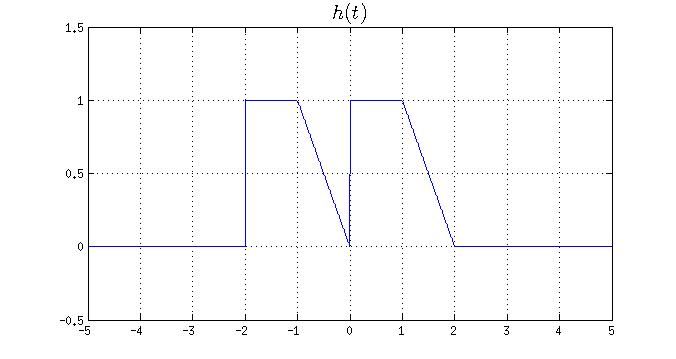
\includegraphics[width=0.80\textwidth]{./lab2prob7.png}
            \end{center}
        \end{figure}

        \begin{enumerate}
            \item $h\left(t+1\right)$
            \item $h\left(\frac{t}{2}-2\right)$
            \item $h\left(1-2t\right)$
            \item $4h\left(\frac{t}{4}\right)$
            \item $\frac{1}{2}h\left(t\right)u\left(t\right) + h\left(-t\right)u\left(t\right)$
            \item $h\left(\frac{t}{2}\right)\delta\left(t+1\right)$
            \item $h\left(t\right)\left(u\left(t+1\right)-u\left(t-1\right)\right)$
        \end{enumerate}
    \end{enumerate}

\end{document}

